\newpage
\subsection{Caso d'uso UC14: Amministrazione applicazione web}
\label{UC14}
\begin{figure}[ht]
	\centering
	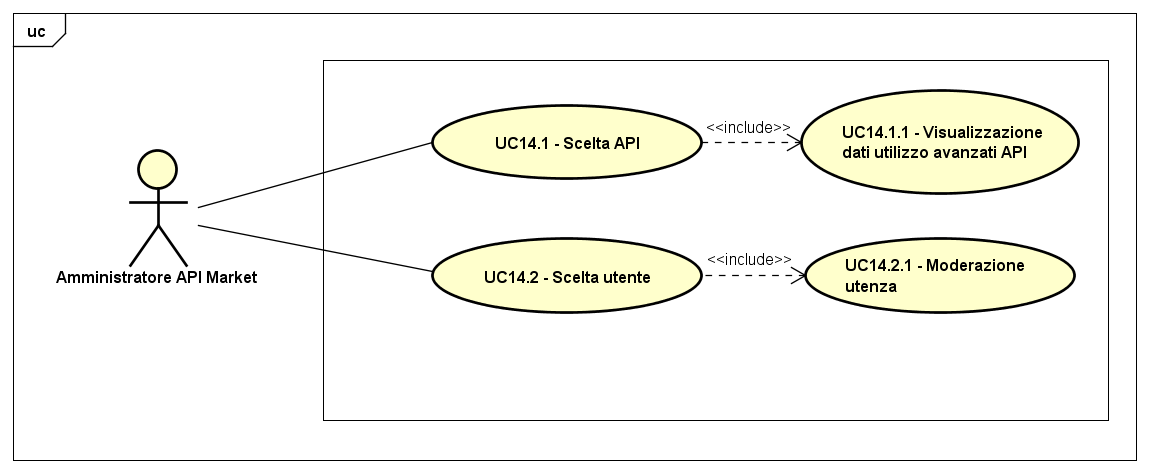
\includegraphics[scale=0.45]{UML/UC14.png}
	\caption{UC14 - Amministrazione applicazione web}
\end{figure}

\begin{longtable}{ l | p{11cm}}
	\hline
	\rowcolor{Gray}
	\multicolumn{2}{c}{UC14: Amministrazione applicazione web} \\
	\hline
	\textbf{Attori} & Amministratore API Market \\
	\textbf{Descrizione} & L'attore amministra l'applicazione web e/o consulta i dati di utilizzo avanzati \\
	\textbf{Pre-Condizioni} & L'attore si trova nella schermata iniziale dell'applicazione web \\
	\textbf{Post-Condizioni} & L'attore ha amministrato l'applicazione web e/o ha consultato i dati di utilizzo avanzati \\
	\textbf{Scenario Principale} & 
	\begin{enumerate*}[label=(\arabic*.),itemjoin={\newline}]
		\item L'attore può scegliere una API (UC14.1) per eseguire delle operazioni su di essa (UC14.1.1)
		\item L'attore può scegliere un utente (UC14.2) da moderare (UC14.2.1)
	\end{enumerate*}\\
\end{longtable}

\subsubsection{Caso d'uso UC14.1: Scelta API}
\label{UC14_1}

\begin{minipage}{\linewidth}
	\begin{tabular}{ l | p{11cm}}
		\hline
		\rowcolor{Gray}
		\multicolumn{2}{c}{UC14.1 - Scelta API} \\
		\hline
		\textbf{Attori} & Amministratore API Market \\
		\textbf{Descrizione} & L'attore sceglie una API su cui effettuare delle operazioni \\
		\textbf{Pre-Condizioni} & L'attore si trova nella schermata relativa all'amministrazione dell'applicazione web \\
		\textbf{Post-Condizioni} & L'attore ha scelto una API su cui effettuare delle operazioni \\
		\textbf{Scenario Principale} & 
		\begin{enumerate*}[label=(\arabic*.),itemjoin={\newline}]
			\item L'attore può scegliere una API su cui effettuare delle operazioni (UC14.1.1)
		\end{enumerate*}\\
	\end{tabular}
\end{minipage}

\newpage
\subsubsection{Caso d'uso UC14.1.1: Operazioni su API}
\label{UC14_1_1}
\begin{figure}[ht]
	\centering
	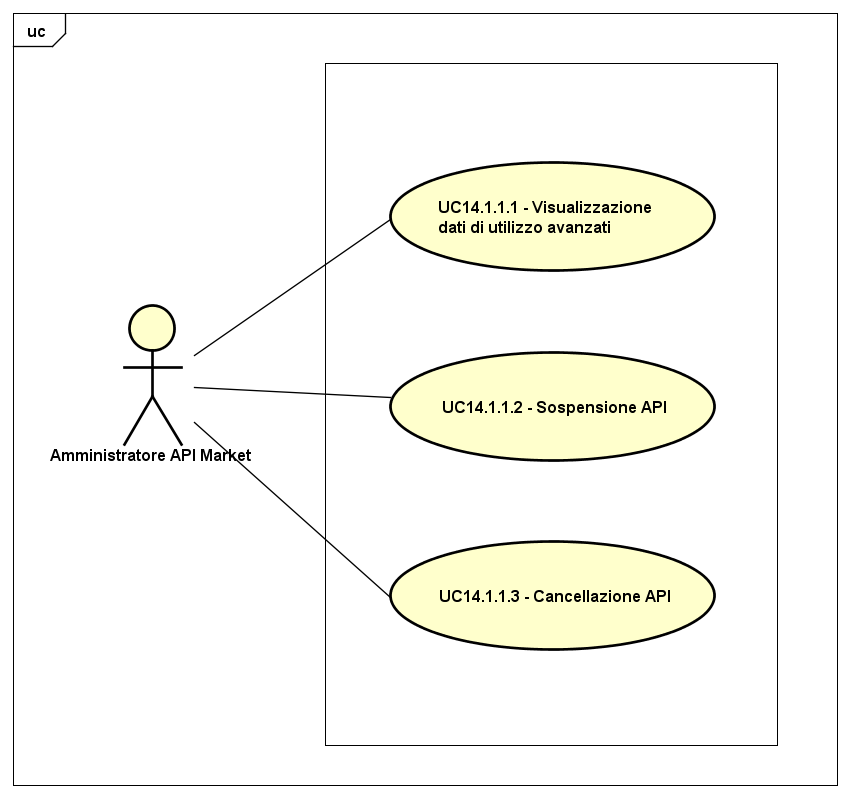
\includegraphics[scale=0.45]{UML/UC14_1_1.png}
	\caption{UC14.1.1: Operazioni su API}
\end{figure}

\begin{minipage}{\linewidth}
	\begin{tabular}{ l | p{11cm}}
		\hline
		\rowcolor{Gray}
		\multicolumn{2}{c}{UC14.1.1 - Operazioni su API} \\
		\hline
		\textbf{Attori} &  Amministratore API Market \\
		\textbf{Descrizione} & L'attore esegue le operazioni sull'API \\
		\textbf{Pre-Condizioni} & L'attore si trova nella schermata relativa all'amministrazione dell'applicazione web \\
		\textbf{Post-Condizioni} & L'attore ha concluso le operazioni sull'API \\
		\textbf{Scenario Principale} & 
		\begin{enumerate*}[label=(\arabic*.),itemjoin={\newline}]
			\item L'attore può visualizzare i dati avanzati dell'API (UC14.1.1.1)
			\item L'attore può sospendere il funzionamento dell'API (UC14.1.1.2)
			\item L'attore può cancellare l'API da API Market (UC14.1.1.3)
		\end{enumerate*}\\
	\end{tabular}
\end{minipage}

\newpage
\subsubsection{Caso d'uso UC14.1.1.1: Visualizzazione dati di utilizzo avanzati}
\label{UC14_1_1_1}
\begin{figure}[ht]
	\centering
	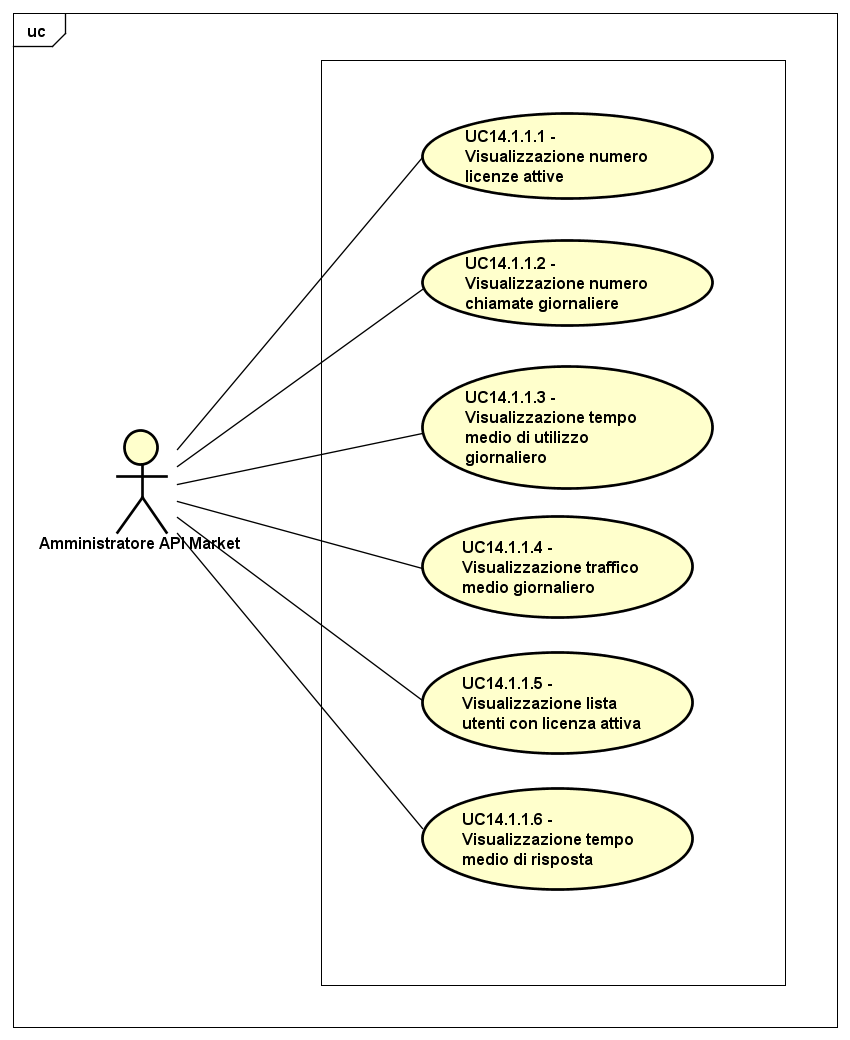
\includegraphics[scale=0.45]{UML/UC14_1_1_1.png}
	\caption{UC14.1.1: Visualizzazione dati di utilizzo avanzati}
\end{figure}

\begin{minipage}{\linewidth}
	\begin{tabular}{ l | p{11cm}}
		\hline
		\rowcolor{Gray}
		\multicolumn{2}{c}{UC14.1.1.1 - Visualizzazione dati di utilizzo avanzati} \\
		\hline
		\textbf{Attori} &  Amministratore API Market \\
		\textbf{Descrizione} & L'attore sceglie una API e ne visualizza i dati di utilizzo avanzati \\
		\textbf{Pre-Condizioni} & L'attore si trova nella schermata relativa all'amministrazione dell'applicazione web \\
		\textbf{Post-Condizioni} & L'attore ha scelto una API e ne ha visualizzato i dati di utilizzo avanzati \\
		\textbf{Scenario Principale} & 
		\begin{enumerate*}[label=(\arabic*.),itemjoin={\newline}]
			\item L'attore può visualizzare il numero di licenze attive dell'API scelta (UC14.1.1.1)
			\item L'attore può visualizzare il numero di chiamate giornaliere effettuate all'API scelta (UC14.1.1.2)
			\item L'attore può visualizzare il tempo medio di utilizzo giornaliero dell'API scelta (UC14.1.1.3)
			\item L'attore può visualizzare il traffico medio giornaliero dell'API scelta (UC14.1.1.4)
			\item L'attore può visualizzare la lista degli utenti con una licenza attiva per l'API scelta (UC14.1.1.5)
			\item L'attore può visualizzare il tempo medio di risposta dell'API scelta (UC14.1.1.6)
		\end{enumerate*}\\
	\end{tabular}
\end{minipage}

\paragraph{Caso d'uso UC14.1.1.1: Visualizzazione numero licenze attive}
\label{UC14_1_1_1}

\begin{minipage}{\linewidth}
	\begin{tabular}{ l | p{11cm}}
		\hline
		\rowcolor{Gray}
		\multicolumn{2}{c}{UC14.1.1.1 - Visualizzazione numero licenze attive} \\
		\hline
		\textbf{Attori} & Amministratore API Market \\
		\textbf{Descrizione} & L'attore visualizza il numero di licenze attive per l'API scelta \\
		\textbf{Pre-Condizioni} & L'attore si trova nella schermata di visualizzazione dati di utilizzo API avanzati ed ha scelto una API \\
		\textbf{Post-Condizioni} & L'attore ha visualizzato il numero di licenze attive per l'API scelta \\
		\textbf{Scenario Principale} & 
		\begin{enumerate*}[label=(\arabic*.),itemjoin={\newline}]
			\item L'attore può visualizzare il numero di licenze attive per l'API scelta
		\end{enumerate*}\\
	\end{tabular}
\end{minipage}

\paragraph{Caso d'uso UC14.1.1.2: Visualizzazione numero chiamate giornaliere}
\label{UC14_1_1_2}

\begin{minipage}{\linewidth}
	\begin{tabular}{ l | p{11cm}}
		\hline
		\rowcolor{Gray}
		\multicolumn{2}{c}{UC14.1.1.2 - Visualizzazione numero chiamate giornaliere} \\
		\hline
		\textbf{Attori} & Amministratore API Market \\
		\textbf{Descrizione} & L'attore visualizza il numero di chiamate giornaliere effettuate all'API scelta \\
		\textbf{Pre-Condizioni} & L'attore si trova nella schermata di visualizzazione dati di utilizzo API avanzati ed ha scelto una API \\
		\textbf{Post-Condizioni} & L'attore ha visualizzato il numero di chiamate giornaliere effettuate all'API scelta \\
		\textbf{Scenario Principale} & 
		\begin{enumerate*}[label=(\arabic*.),itemjoin={\newline}]
			\item L'attore può visualizzare il numero di chiamate giornaliere effettuate all'API scelta
		\end{enumerate*}\\
	\end{tabular}
\end{minipage}

\paragraph{Caso d'uso UC14.1.1.3: Visualizzazione tempo medio di utilizzo giornaliero}
\label{UC14_1_1_3}

\begin{minipage}{\linewidth}
	\begin{tabular}{ l | p{11cm}}
		\hline
		\rowcolor{Gray}
		\multicolumn{2}{c}{14.1.1.3 - Visualizzazione tempo medio di utilizzo giornaliero} \\
		\hline
		\textbf{Attori} & Amministratore API Market \\
		\textbf{Descrizione} & L'attore visualizza il tempo medio di utilizzo giornaliero dell'API scelta \\
		\textbf{Pre-Condizioni} & L'attore si trova nella schermata di visualizzazione dati di utilizzo API avanzati ed ha scelto una API \\
		\textbf{Post-Condizioni} & L'attore ha visualizzato il tempo medio di utilizzo giornaliero dell'API scelta \\
		\textbf{Scenario Principale} & 
		\begin{enumerate*}[label=(\arabic*.),itemjoin={\newline}]
			\item L'attore può visualizzare il tempo medio di utilizzo giornaliero dell'API scelta
		\end{enumerate*}\\
	\end{tabular}
\end{minipage}

\paragraph{Caso d'uso UC14.1.1.4: Visualizzazione traffico medio giornaliero}
\label{UC14_1_1_4}

\begin{minipage}{\linewidth}
	\begin{tabular}{ l | p{11cm}}
		\hline
		\rowcolor{Gray}
		\multicolumn{2}{c}{UC14.1.1.4 - Visualizzazione traffico medio giornaliero} \\
		\hline
		\textbf{Attori} & Amministratore API Market \\
		\textbf{Descrizione} & L'attore visualizza il traffico medio giornaliero dell'API scelta \\
		\textbf{Pre-Condizioni} & L'attore si trova nella schermata di visualizzazione dati di utilizzo API avanzati ed ha scelto una API \\
		\textbf{Post-Condizioni} & L'attore ha visualizzato il traffico medio giornaliero dell'API scelta \\
		\textbf{Scenario Principale} & 
		\begin{enumerate*}[label=(\arabic*.),itemjoin={\newline}]
			\item L'attore può visualizzare il traffico medio giornaliero dell'API scelta
		\end{enumerate*}\\
	\end{tabular}
\end{minipage}

\newpage
\paragraph{Caso d'uso UC14.1.1.1.5: Visualizzazione utenti con licenza attiva}
\label{UC14_1_1_1_5}
\begin{figure}[ht]
	\centering
	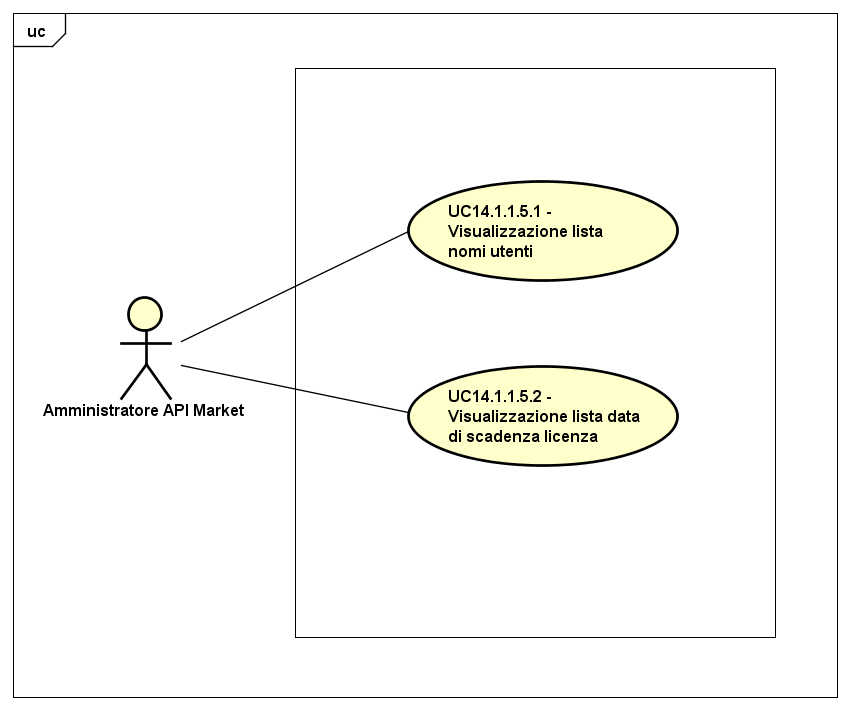
\includegraphics[scale=0.45]{UML/UC14_1_1_1_5.png}
	\caption{UC14.1.1.5: Visualizzazione utenti con licenza attiva}
\end{figure}

\begin{minipage}{\linewidth}
	\begin{tabular}{ l | p{11cm}}
		\hline
		\rowcolor{Gray}
		\multicolumn{2}{c}{UC14.1.1.1.5 - Visualizzazione utenti con licenza attiva} \\
		\hline
		\textbf{Attori} & Amministratore API Market \\
		\textbf{Descrizione} & L'attore ha scelto una API e visualizza una lista di utenti con licenze attive per l'API scelta\\
		\textbf{Pre-Condizioni} & L'attore si trova nella schermata di visualizzazione dati di utilizzo API avanzati ed ha scelto una API \\
		\textbf{Post-Condizioni} & L'attore ha visualizzato la lista di utenti con licenze attive per l'API scelta \\
		\textbf{Scenario Principale} & 
		\begin{enumerate*}[label=(\arabic*.),itemjoin={\newline}]
			\item L'attore può visualizzare il nome di ogni utente con licenza attiva per l'API scelta (UC14.1.1.5.1)
			\item L'attore può visualizzare la data di scadenza della licenza per ogni utente nella lista (UC14.1.1.5.2)
		\end{enumerate*}\\
	\end{tabular}
\end{minipage}

\subparagraph{Caso d'uso UC14.1..11.5.1: Visualizzazione lista nomi utenti}
\label{UC14_1_1_1_5_1}

\begin{minipage}{\linewidth}
	\begin{tabular}{ l | p{11cm}}
		\hline
		\rowcolor{Gray}
		\multicolumn{2}{c}{UC14.1.1.1.5.1 - Visualizzazione lista nomi utenti} \\
		\hline
		\textbf{Attori} & Amministratore API Market \\
		\textbf{Descrizione} & L'attore ha scelto una API e visualizza il nome dell'utente interessato\\
		\textbf{Pre-Condizioni} & L'attore si trova nella schermata di visualizzazione dati di utilizzo API avanzati ed ha scelto una API \\
		\textbf{Post-Condizioni} & L'attore ha visualizzato il nome per ogni utente della lista degli utenti con licenza attiva per l'API scelta \\
		\textbf{Scenario Principale} & 
		\begin{enumerate*}[label=(\arabic*.),itemjoin={\newline}]
			\item L'attore può visualizzare il nome per ogni utente della lista degli utenti con licenza attiva per l'API scelta
		\end{enumerate*}
	\end{tabular}
\end{minipage}

\subparagraph{Caso d'uso UC14.1.1.1.5.2: Visualizzazione lista data di scadenza licenza}
\label{UC14_1_1_1_5_2}

\begin{minipage}{\linewidth}
	\begin{tabular}{ l | p{11cm}}
		\hline
		\rowcolor{Gray}
		\multicolumn{2}{c}{UC14.1.1.1.5.2 -  Visualizzazione lista data di scadenza licenza} \\
		\hline
		\textbf{Attori} & Amministratore API Market \\
		\textbf{Descrizione} & L'attore ha scelto una API e visualizza la data di scadenza per ogni utente della lista degli utenti con licenza attiva per l'API scelta \\
		\textbf{Pre-Condizioni} & L'attore si trova nella schermata di visualizzazione dati di utilizzo API avanzati ed ha scelto una API \\
		\textbf{Post-Condizioni} & L'attore ha visualizzato la data di scadenza per ogni utente della lista degli utenti con licenza attiva per l'API scelta \\
		\textbf{Scenario Principale} & 
		\begin{enumerate*}[label=(\arabic*.),itemjoin={\newline}]
			\item L'attore può visualizzare la data di scadenza per ogni utente della lista degli utenti con licenza attiva per l'API scelta
		\end{enumerate*}
	\end{tabular}
\end{minipage}

\paragraph{Caso d'uso UC14.1.1.1.6: Visualizzazione tempo medio di risposta}
\label{UC14_1_1_1_6}

\begin{minipage}{\linewidth}
	\begin{tabular}{ l | p{11cm}}
		\hline
		\rowcolor{Gray}
		\multicolumn{2}{c}{UC14.1.1.1.6 - Visualizzazione tempo medio di risposta} \\
		\hline
		\textbf{Attori} & Amministratore API Market \\
		\textbf{Descrizione} & L'attore ha scelto una API e visualizza il tempo medio di risposta dell'API scelta \\
		\textbf{Pre-Condizioni} & L'attore si trova nella schermata di visualizzazione dati di utilizzo API avanzati ed ha scelto una API \\
		\textbf{Post-Condizioni} & L'attore ha visualizzato il tempo medio di risposta dell'API scelta \\
		\textbf{Scenario Principale} & 
		\begin{enumerate*}[label=(\arabic*.),itemjoin={\newline}]
			\item L'attore può visualizzare il tempo medio di risposta dell'API scelta
		\end{enumerate*}\\
	\end{tabular}
\end{minipage}

\newpage
\paragraph{Caso d'uso UC14.1.1.2: Sospensione API}
\label{UC14_1_1_2}
\begin{figure}[ht]
	\centering
	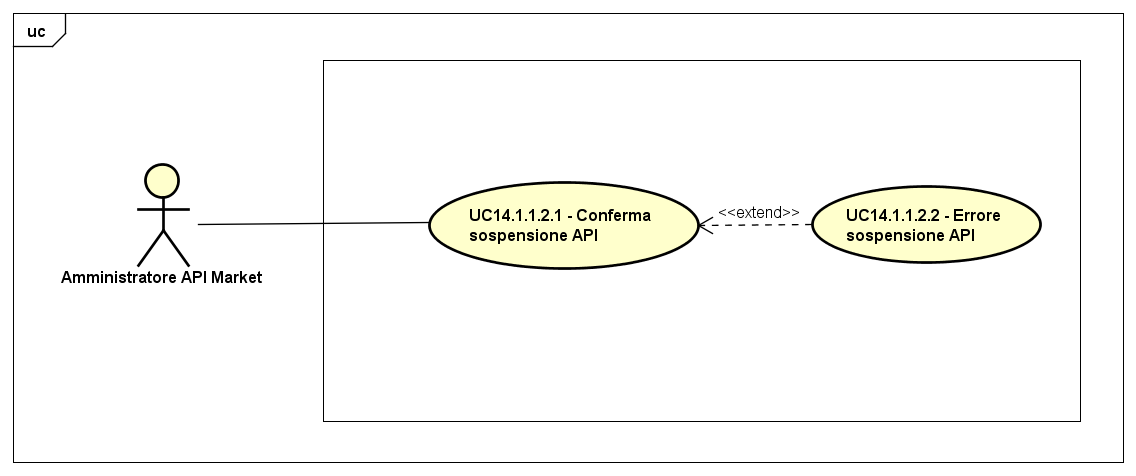
\includegraphics[scale=0.45]{UML/UC14_1_1_2.png}
	\caption{UC14.1.1.2: Sospensione API}
\end{figure}

\begin{minipage}{\linewidth}
	\begin{tabular}{ l | p{11cm}}
		\hline
		\rowcolor{Gray}
		\multicolumn{2}{c}{UC14.1.1.2 - Sospensione API} \\
		\hline
		\textbf{Attori} & Amministratore API Market \\
		\textbf{Descrizione} & L'attore sospende l'API scelta \\
		\textbf{Pre-Condizioni} & L'attore si trova nella schermata relativa alle operazioni su API ed ha scelto una API \\
		\textbf{Post-Condizioni} & L'attore ha sospeso l'API scelta \\
		\textbf{Scenario Principale} & 
		\begin{enumerate*}[label=(\arabic*.),itemjoin={\newline}]
			\item L'attore può confermare la sospensione dell'API scelta (UC14.1.1.2.1)
		\end{enumerate*}\\
		\textbf{Scenari Alternativi} & 
		\begin{enumerate*}[label=(\arabic*.),itemjoin={\newline}]
			\item L'attore può visualizzare un messaggio di errore informativo e la sospensione dell'API scelta non avviene (UC14.1.1.2.2)
		\end{enumerate*}\\
	\end{tabular}
\end{minipage}

\subparagraph{Caso d'uso UC14.1.1.2.1: Conferma sospensione API}
\label{UC14_1_1_2_1}

\begin{minipage}{\linewidth}
	\begin{tabular}{ l | p{11cm}}
		\hline
		\rowcolor{Gray}
		\multicolumn{2}{c}{UC14.1.1.2.1 - Conferma sospensione API} \\
		\hline
		\textbf{Attori} & Amministratore API Market \\
		\textbf{Descrizione} & L'attore conferma la sospensione dell'utente scelto e visualizza un messaggio di successo \\
		\textbf{Pre-Condizioni} & L'attore si trova nella schermata relativa alle operazioni su API ed ha scelto una API \\
		\textbf{Post-Condizioni} & L'attore ha confermato la sospensione dell'API scelta \\
		\textbf{Scenario Principale} & 
		\begin{enumerate*}[label=(\arabic*.),itemjoin={\newline}]
			\item L'attore conferma la sospensione dell'API scelta e visualizza un messaggio di successo
		\end{enumerate*}\\
	\end{tabular}
\end{minipage}

\subparagraph{Caso d'uso UC14.1.1.2.2: Errore sospensione API}
\label{UC14_1_1_2_2}

\begin{minipage}{\linewidth}
	\begin{tabular}{ l | p{11cm}}
		\hline
		\rowcolor{Gray}
		\multicolumn{2}{c}{UC14.1.1.2.2 - Errore sospensione API} \\
		\hline
		\textbf{Attori} & Amministratore API Market \\
		\textbf{Descrizione} & L'attore visualizza un messaggio di errore informativo e la sospensione dell'API scelta non avviene \\
		\textbf{Pre-Condizioni} & L'attore ha confermato la sospensione dell'API scelta ma si è verificato un errore \\
		\textbf{Post-Condizioni} & L'attore ha visualizzato un messaggio di errore informativo \\
		\textbf{Scenario Principale} & 
		\begin{enumerate*}[label=(\arabic*.),itemjoin={\newline}]
			\item L'attore può visualizzare un messaggio di errore informativo e la sospensione dell'API scelta non avviene
		\end{enumerate*}\\
	\end{tabular}
\end{minipage}

\newpage
\paragraph{Caso d'uso UC14.1.1.3: Cancellazione API}
\label{UC14_1_1_3}
\begin{figure}[ht]
	\centering
	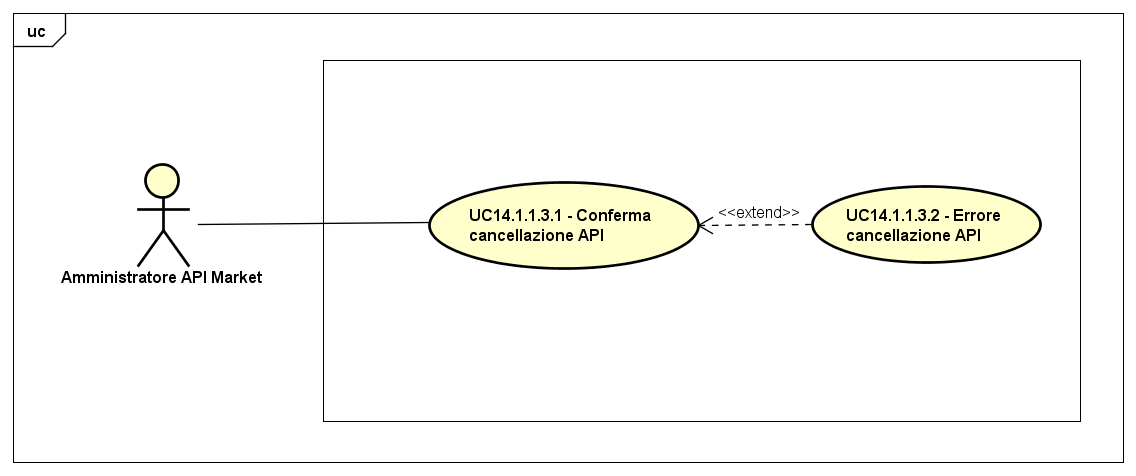
\includegraphics[scale=0.45]{UML/UC14_1_1_3.png}
	\caption{UC14.1.1.3: Cancellazione API}
\end{figure}

\begin{minipage}{\linewidth}
	\begin{tabular}{ l | p{11cm}}
		\hline
		\rowcolor{Gray}
		\multicolumn{2}{c}{UC14.1.1.3 - Cancellazione API} \\
		\hline
		\textbf{Attori} & Amministratore API Market \\
		\textbf{Descrizione} & L'attore cancella l'API scelta \\
		\textbf{Pre-Condizioni} & L'attore si trova nella schermata relativa alle operazioni su API ed ha scelto una API \\
		\textbf{Post-Condizioni} & L'attore ha cancellato l'API scelta \\
		\textbf{Scenario Principale} & 
		\begin{enumerate*}[label=(\arabic*.),itemjoin={\newline}]
			\item L'attore può confermare la cancellazione dell'API scelta (UC14.1.1.3.1)
		\end{enumerate*}\\
		\textbf{Scenari Alternativi} & 
		\begin{enumerate*}[label=(\arabic*.),itemjoin={\newline}]
			\item L'attore può visualizzare un messaggio di errore informativo e la cancellazione dell'API scelta non avviene (UC14.1.1.3.2)
		\end{enumerate*}\\
	\end{tabular}
\end{minipage}

\subparagraph{Caso d'uso UC14.1.1.3.1: Conferma cancellazione API}
\label{UC14_1_1_3_1}

\begin{minipage}{\linewidth}
	\begin{tabular}{ l | p{11cm}}
		\hline
		\rowcolor{Gray}
		\multicolumn{2}{c}{UC14.1.1.3.1 - Conferma cancellazione API} \\
		\hline
		\textbf{Attori} & Amministratore API Market \\
		\textbf{Descrizione} & L'attore conferma la cancellazione dell'utente scelto e visualizza un messaggio di successo \\
		\textbf{Pre-Condizioni} & L'attore si trova nella schermata relativa alle operazioni su API ed ha scelto una API \\
		\textbf{Post-Condizioni} & L'attore ha confermato la cancellazione dell'API scelta \\
		\textbf{Scenario Principale} & 
		\begin{enumerate*}[label=(\arabic*.),itemjoin={\newline}]
			\item L'attore conferma la cancellazione dell'API scelta e visualizza un messaggio di successo
		\end{enumerate*}\\
	\end{tabular}
\end{minipage}

\subparagraph{Caso d'uso UC14.1.1.3.2: Errore cancellazione API}
\label{UC14_1_1_3_2}

\begin{minipage}{\linewidth}
	\begin{tabular}{ l | p{11cm}}
		\hline
		\rowcolor{Gray}
		\multicolumn{2}{c}{UC14.1.1.3.2 - Errore cancellazione API} \\
		\hline
		\textbf{Attori} & Amministratore API Market \\
		\textbf{Descrizione} & L'attore visualizza un messaggio di errore informativo e la cancellazione dell'API scelta non avviene \\
		\textbf{Pre-Condizioni} & L'attore ha confermato la cancellazione dell'API scelta ma si è verificato un errore \\
		\textbf{Post-Condizioni} & L'attore ha visualizzato un messaggio di errore informativo \\
		\textbf{Scenario Principale} & 
		\begin{enumerate*}[label=(\arabic*.),itemjoin={\newline}]
			\item L'attore può visualizzare un messaggio di errore informativo e la cancellazione dell'API scelta non avviene
		\end{enumerate*}\\
	\end{tabular}
\end{minipage}

\subsubsection{Caso d'uso UC14.2.1: Scelta utente}
\label{UC14_2_1}

\begin{minipage}{\linewidth}
	\begin{tabular}{ l | p{11cm}}
		\hline
		\rowcolor{Gray}
		\multicolumn{2}{c}{UC14.2.1 - Scelta utente} \\
		\hline
		\textbf{Attori} & Amministratore API Market \\
		\textbf{Descrizione} & L'attore sceglie un utente da moderare \\
		\textbf{Pre-Condizioni} & L'attore si trova nella schermata relativa all'amministrazione dell'applicazione web \\
		\textbf{Post-Condizioni} & L'attore ha scelto un utente da moderare \\
		\textbf{Scenario Principale} & 
		\begin{enumerate*}[label=(\arabic*.),itemjoin={\newline}]
			\item L'attore può scegliere un utente da moderare (UC14.2.1.1)
		\end{enumerate*}\\
	\end{tabular}
\end{minipage}

\newpage
\subsubsection{Caso d'uso UC14.2.1: Moderazione utenza}
\label{UC14_2_1}
\begin{figure}[ht]
	\centering
	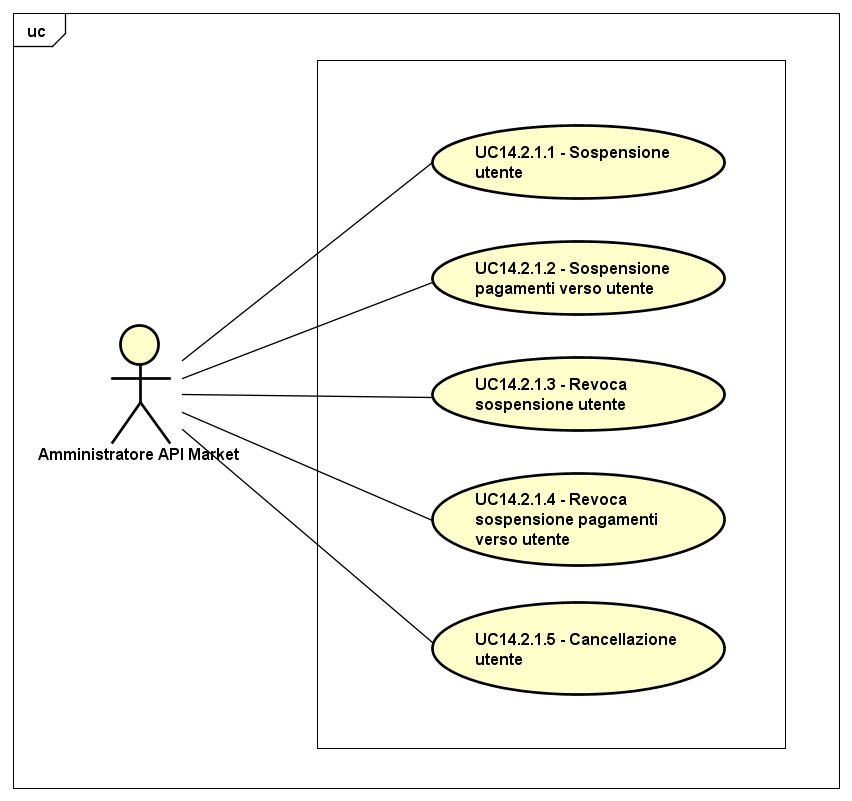
\includegraphics[scale=0.45]{UML/UC14_2_1.png}
	\caption{UC14.2.1: Moderazione utenza}
\end{figure}

\begin{minipage}{\linewidth}
	\begin{tabular}{ l | p{11cm}}
		\hline
		\rowcolor{Gray}
		\multicolumn{2}{c}{UC14.2.1 - Moderazione utenza} \\
		\hline
		\textbf{Attori} &  Amministratore API Market \\
		\textbf{Descrizione} & L'attore attua l'opera di moderazione \\
		\textbf{Pre-Condizioni} & L'attore si trova nella schermata relativa all'amministrazione dell'applicazione web \\
		\textbf{Post-Condizioni} & L'attore ha concluso l'opera di moderazione \\
		\textbf{Scenario Principale} & 
		\begin{enumerate*}[label=(\arabic*.),itemjoin={\newline}]
			\item L'attore può sospendere l'utente scelto (UC14.2.1.1)
			\item L'attore può sospendere i pagamenti verso l'utente scelto (UC14.2.1.2)
			\item L'attore può revocare la sospensione dell'utente scelto (UC14.2.1.3)
			\item L'attore può revocare la sospensione dei pagamenti verso l'utente scelto (UC14.2.1.4)
		\end{enumerate*}\\
	\end{tabular}
\end{minipage}

\newpage
\paragraph{Caso d'uso UC14.2.1.1: Sospensione utente}
\label{UC14_2_1_1}
\begin{figure}[ht]
	\centering
	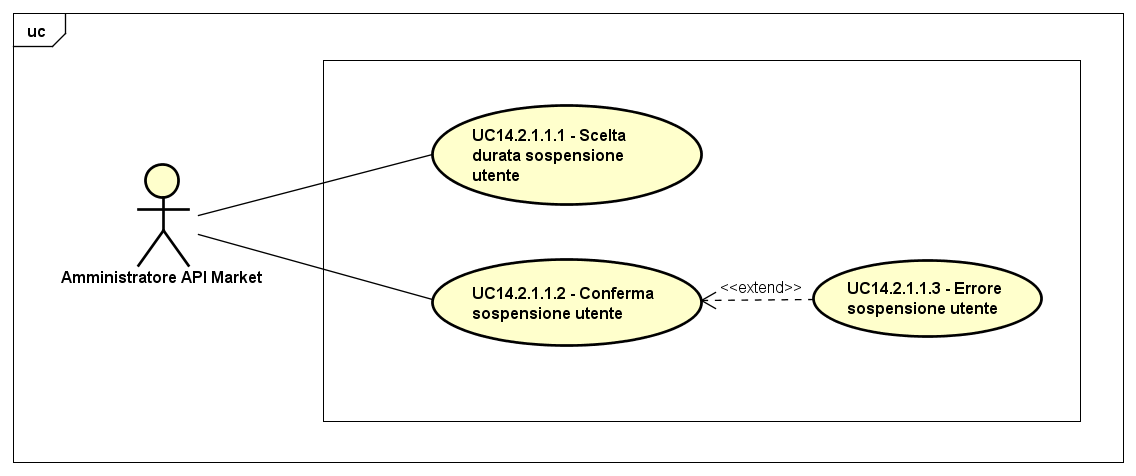
\includegraphics[scale=0.45]{UML/UC14_2_1_1.png}
	\caption{UC14.2.1.1: Sospensione utente}
\end{figure}

\begin{minipage}{\linewidth}
	\begin{tabular}{ l | p{11cm}}
		\hline
		\rowcolor{Gray}
		\multicolumn{2}{c}{UC14.2.1.1 - Sospensione utente} \\
		\hline
		\textbf{Attori} & Amministratore API Market \\
		\textbf{Descrizione} & L'attore sospende l'utente scelto (impedisce da parte sua l'uso delle API acquistate, e da parte degli altri utente l'uso delle API da lui registrate) \\
		\textbf{Pre-Condizioni} & L'attore si trova nella schermata relativa alla moderazione dell'utenza ed ha scelto un utente \\
		\textbf{Post-Condizioni} & L'attore ha sospeso l'utente scelto \\
		\textbf{Scenario Principale} & 
		\begin{enumerate*}[label=(\arabic*.),itemjoin={\newline}]
			\item L'attore può confermare la sospensione dell'utente scelto (UC14.2.1.1.1)
		\end{enumerate*}\\
		\textbf{Scenari Alternativi} & 
		\begin{enumerate*}[label=(\arabic*.),itemjoin={\newline}]
			\item L'attore può visualizzare un messaggio di errore informativo e la sospensione dell'utente scelto non avviene (UC14.2.1.1.2)
		\end{enumerate*}\\
	\end{tabular}
\end{minipage}

\subparagraph{Caso d'uso UC14.2.1.1.1: Conferma sospensione utente}
\label{UC14_2_1_1_1}

\begin{minipage}{\linewidth}
	\begin{tabular}{ l | p{11cm}}
		\hline
		\rowcolor{Gray}
		\multicolumn{2}{c}{UC14.2.1.1.1 - Conferma sospensione utente} \\
		\hline
		\textbf{Attori} & Amministratore API Market \\
		\textbf{Descrizione} & L'attore conferma la sospensione dell'utente scelto e visualizza un messaggio di successo \\
		\textbf{Pre-Condizioni} & L'attore si trova nella schermata relativa alla moderazione dell'utenza ed ha scelto un utente \\
		\textbf{Post-Condizioni} & L'attore ha confermato la sospensione dell'utente scelto \\
		\textbf{Scenario Principale} & 
		\begin{enumerate*}[label=(\arabic*.),itemjoin={\newline}]
			\item L'attore conferma la sospensione dell'utente scelto e visualizza un messaggio di successo
		\end{enumerate*}\\
	\end{tabular}
\end{minipage}

\subparagraph{Caso d'uso UC14.2.1.1.2: Errore sospensione utente}
\label{UC14_2_1_1_2}

\begin{minipage}{\linewidth}
	\begin{tabular}{ l | p{11cm}}
		\hline
		\rowcolor{Gray}
		\multicolumn{2}{c}{UC14.2.1.1.2 - Errore sospensione utente} \\
		\hline
		\textbf{Attori} & Amministratore API Market \\
		\textbf{Descrizione} & L'attore visualizza un messaggio di errore informativo e la sospensione dell'utente scelto non avviene \\
		\textbf{Pre-Condizioni} & L'attore ha confermato la sospensione dell'utente scelto ma si è verificato un errore \\
		\textbf{Post-Condizioni} & L'attore ha visualizzato un messaggio di errore informativo \\
		\textbf{Scenario Principale} & 
		\begin{enumerate*}[label=(\arabic*.),itemjoin={\newline}]
			\item L'attore può visualizzare un messaggio di errore informativo e la sospensione dell'utente scelto non avviene
		\end{enumerate*}\\
	\end{tabular}
\end{minipage}

\newpage
\paragraph{Caso d'uso UC14.2.1.2: Sospensione prelievi conto utente}
\label{UC14_2_1_2}
\begin{figure}[ht]
	\centering
	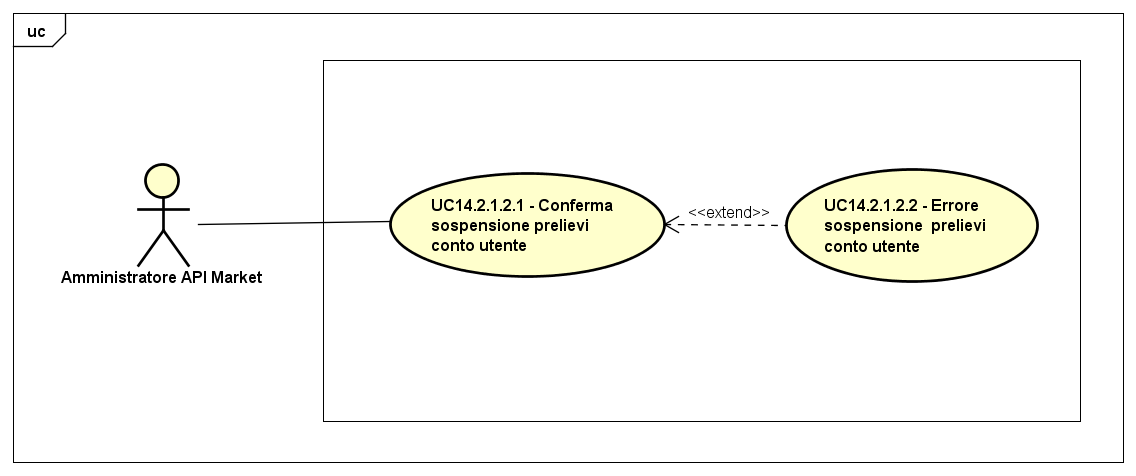
\includegraphics[scale=0.45]{UML/UC14_2_1_2.png}
	\caption{UC14.2.1.2: Sospensione prelievi conto utente}
\end{figure}

\begin{minipage}{\linewidth}
	\begin{tabular}{ l | p{11cm}}
		\hline
		\rowcolor{Gray}
		\multicolumn{2}{c}{UC14.2.1.2 - Sospensione prelievi conto utente} \\
		\hline
		\textbf{Attori} & Amministratore API Market \\
		\textbf{Descrizione} & L'attore sospende i pagamenti verso l'utente scelto \\
		\textbf{Pre-Condizioni} & L'attore si trova nella schermata relativa alla moderazione dell'utenza ed ha scelto un utente \\
		\textbf{Post-Condizioni} & L'attore ha sospeso i pagamenti verso l'utente scelto \\
		\textbf{Scenario Principale} & 
		\begin{enumerate*}[label=(\arabic*.),itemjoin={\newline}]
			\item L'attore può sospendere i pagamenti verso l'utente scelto (UC14.2.1.2.1)
		\end{enumerate*}\\
		\textbf{Scenari Alternativi} & 
		\begin{enumerate*}[label=(\arabic*.),itemjoin={\newline}]
			\item L'attore può visualizzare un messaggio di errore informativo e la sospensione i pagamenti verso l'utente scelto non avviene (UC14.2.1.2.2)
		\end{enumerate*}\\
	\end{tabular}
\end{minipage}

\subparagraph{Caso d'uso UC14.2.1.2.1: Conferma sospensione pagamenti verso utente}
\label{UC14_2_1_2_1}

\begin{minipage}{\linewidth}
	\begin{tabular}{ l | p{11cm}}
		\hline
		\rowcolor{Gray}
		\multicolumn{2}{c}{UC14.2.1.2.1 - Conferma sospensione pagamenti verso utente} \\
		\hline
		\textbf{Attori} & Amministratore API Market \\
		\textbf{Descrizione} & L'attore conferma la sospensione dei pagamenti verso l'utente scelto e visualizza un messaggio di successo \\
		\textbf{Pre-Condizioni} & L'attore si trova nella schermata relativa alla moderazione dell'utenza ed ha scelto un utente \\
		\textbf{Post-Condizioni} & L'attore ha confermato la sospensione dei pagamenti verso l'utente scelto \\
		\textbf{Scenario Principale} & 
		\begin{enumerate*}[label=(\arabic*.),itemjoin={\newline}]
			\item L'attore conferma la sospensione dei pagamenti verso l'utente scelto e visualizza un messaggio di successo
		\end{enumerate*}\\
	\end{tabular}
\end{minipage}

\subparagraph{Caso d'uso UC14.2.1.2.2: Errore sospensione pagamenti verso utente}
\label{UC14_2_1_2_2}

\begin{minipage}{\linewidth}
	\begin{tabular}{ l | p{11cm}}
		\hline
		\rowcolor{Gray}
		\multicolumn{2}{c}{UC14.2.1.2.2 - Errore sospensione pagamenti verso utente} \\
		\hline
		\textbf{Attori} & Amministratore API Market \\
		\textbf{Descrizione} & L'attore visualizza un messaggio di errore informativo e la sospensione dei pagamenti verso l'utente scelto non avviene \\
		\textbf{Pre-Condizioni} & L'attore ha confermato la sospensione dei pagamenti verso l'utente scelto ma si è verificato un errore \\
		\textbf{Post-Condizioni} & L'attore ha visualizzato un messaggio di errore informativo \\
		\textbf{Scenario Principale} & 
		\begin{enumerate*}[label=(\arabic*.),itemjoin={\newline}]
			\item L'attore può visualizzare un messaggio di errore informativo e la sospensione dei pagamenti verso l'utente scelto non avviene
		\end{enumerate*}\\
	\end{tabular}
\end{minipage}

\paragraph{Caso d'uso UC14.2.1.3: Revoca sospensione utente}
\label{UC14_2_1_3}

\begin{minipage}{\linewidth}
	\begin{tabular}{ l | p{11cm}}
		\hline
		\rowcolor{Gray}
		\multicolumn{2}{c}{UC14.2.1.3 - Revoca sospensione utente} \\
		\hline
		\textbf{Attori} & Amministratore API Market \\
		\textbf{Descrizione} & L'attore revoca la sospensione dell'utente scelto, ricevendo un messaggio di successo \\
		\textbf{Pre-Condizioni} & L'attore si trova nella schermata relativa alla moderazione dell'utenza ed ha scelto un utente \\
		\textbf{Post-Condizioni} & L'attore ha revocato la sospensione dell'utente scelto, ricevendo un messaggio di successo \\
		\textbf{Scenario Principale} & 
		\begin{enumerate*}[label=(\arabic*.),itemjoin={\newline}]
			\item L'attore può revocare la sospensione dell'utente scelto, ricevendo un messaggio di successo
		\end{enumerate*}\\
	\end{tabular}
\end{minipage}

\paragraph{Caso d'uso UC14.2.1.4: Revoca sospensione pagamenti verso utente}
\label{UC14_2_1_4}

\begin{minipage}{\linewidth}
	\begin{tabular}{ l | p{11cm}}
		\hline
		\rowcolor{Gray}
		\multicolumn{2}{c}{UC14.2.1.4 - Revoca sospensione pagamenti verso utente} \\
		\hline
		\textbf{Attori} & Amministratore API Market \\
		\textbf{Descrizione} & L'attore revoca la sospensione dei pagamenti verso l'utente scelto, ricevendo un messaggio di successo \\
		\textbf{Pre-Condizioni} & L'attore si trova nella schermata relativa alla moderazione dell'utenza ed ha scelto un utente \\
		\textbf{Post-Condizioni} & L'attore ha revocato la sospensione dei pagamenti verso l'utente scelto, ricevendo un messaggio di successo \\
		\textbf{Scenario Principale} & 
		\begin{enumerate*}[label=(\arabic*.),itemjoin={\newline}]
			\item L'attore può revocare la sospensione dei pagamenti verso l'utente scelto, ricevendo un messaggio di successo
		\end{enumerate*}\\
	\end{tabular}
\end{minipage}

\newpage
\paragraph{Caso d'uso UC14.2.1.5: Cancellazione utente}
\label{UC14_2_1_5}
\begin{figure}[ht]
	\centering
	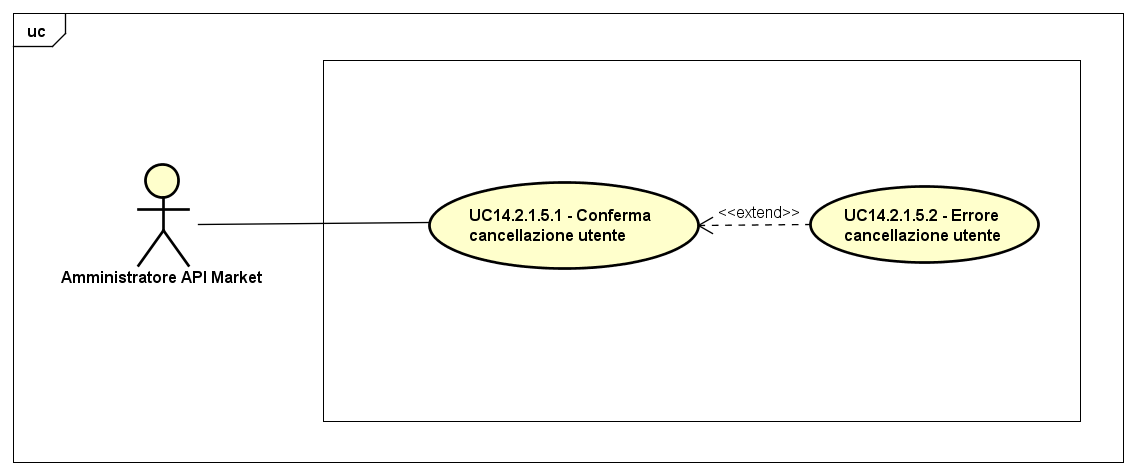
\includegraphics[scale=0.45]{UML/UC14_2_1_5.png}
	\caption{UC14.2.1.5: Cancellazione utente}
\end{figure}

\begin{minipage}{\linewidth}
	\begin{tabular}{ l | p{11cm}}
		\hline
		\rowcolor{Gray}
		\multicolumn{2}{c}{UC14.2.1.5 - Cancellazione utente} \\
		\hline
		\textbf{Attori} & Amministratore API Market \\
		\textbf{Descrizione} & L'attore cancella l'utente scelto \\
		\textbf{Pre-Condizioni} & L'attore si trova nella schermata relativa alla moderazione dell'utenza ed ha scelto un utente \\
		\textbf{Post-Condizioni} & L'attore ha cancellato l'utente scelto \\
		\textbf{Scenario Principale} & 
		\begin{enumerate*}[label=(\arabic*.),itemjoin={\newline}]
			\item L'attore può confermare la cancellazione dell'utente scelto (UC14.2.1.5.1)
		\end{enumerate*}\\
		\textbf{Scenari Alternativi} & 
		\begin{enumerate*}[label=(\arabic*.),itemjoin={\newline}]
			\item L'attore può visualizzare un messaggio di errore informativo e la cancellazione dell'utente scelto non avviene (UC14.2.1.5.2)
		\end{enumerate*}\\
	\end{tabular}
\end{minipage}

\subparagraph{Caso d'uso UC14.2.1.5.1: Conferma cancellazione utente}
\label{UC14_2_1_5_1}

\begin{minipage}{\linewidth}
	\begin{tabular}{ l | p{11cm}}
		\hline
		\rowcolor{Gray}
		\multicolumn{2}{c}{UC14.2.1.5.1 - Conferma cancellazione utente} \\
		\hline
		\textbf{Attori} & Amministratore API Market \\
		\textbf{Descrizione} & L'attore conferma la cancellazione dell'utente scelto e visualizza un messaggio di successo \\
		\textbf{Pre-Condizioni} & L'attore si trova nella schermata relativa alla moderazione dell'utenza ed ha scelto un utente \\
		\textbf{Post-Condizioni} & L'attore ha confermato la cancellazione dell'utente scelto \\
		\textbf{Scenario Principale} & 
		\begin{enumerate*}[label=(\arabic*.),itemjoin={\newline}]
			\item L'attore conferma la cancellazione dell'utente scelto e visualizza un messaggio di successo
		\end{enumerate*}\\
	\end{tabular}
\end{minipage}

\subparagraph{Caso d'uso UC14.2.1.5.2: Errore cancellazione utente}
\label{UC14_2_1_5_2}

\begin{minipage}{\linewidth}
	\begin{tabular}{ l | p{11cm}}
		\hline
		\rowcolor{Gray}
		\multicolumn{2}{c}{UC14.2.1.5.2 - Errore cancellazione utente} \\
		\hline
		\textbf{Attori} & Amministratore API Market \\
		\textbf{Descrizione} & L'attore visualizza un messaggio di errore informativo e la cancellazione dell'utente scelto non avviene \\
		\textbf{Pre-Condizioni} & L'attore ha confermato la cancellazione dell'utente scelto ma si è verificato un errore \\
		\textbf{Post-Condizioni} & L'attore ha visualizzato un messaggio di errore informativo \\
		\textbf{Scenario Principale} & 
		\begin{enumerate*}[label=(\arabic*.),itemjoin={\newline}]
			\item L'attore può visualizzare un messaggio di errore informativo e la cancellazione dell'utente scelto non avviene
		\end{enumerate*}\\
	\end{tabular}
\end{minipage}